%
% bmi design
%

\documentclass[11pt]{article} 
\usepackage[dvips]{graphicx}
\usepackage{times}

\graphicspath{{./}{figs/}} 

\pagestyle{plain}

\addtolength{\hoffset}{-2cm}
\addtolength{\textwidth}{4cm}

\addtolength{\voffset}{-1.5cm}
\addtolength{\textheight}{3cm}

\setlength{\parindent}{0pt}
\setlength{\parskip}{12pt}

\title{BMI Document}
\author{PVFS Development Team}
\date{July 2002}

\begin{document}

\maketitle

\section{TODO}

\begin{itemize}
\item maybe change method nomenclature to module
\end{itemize}

\section{Introduction}

This document describes the design and use of the Buffered Message
Interface (BMI).  BMI is a network abstraction layer that will form the
basis for communication between components of the Parallel Virtual File
System Version 2.  It is a simple message oriented communications
library that includes features that are particularly useful for
low level parallel I/O operations.

All request protocol messages exchanged between clients and
servers in PVFS2 will be transfered using BMI.

Actual file data transfered in PVFS2 will be sent using the flow
interface (see related documents).  The default flow
implementation will also use BMI as an underlying transport, but
advanced implementations may elect to bypass it.

\section{Related Documents}

\begin{itemize}
\item pvfs2-design-storageint: outlines the Trove interface, which
is a low storage device interface used by PVFS2.  
\item pvfs2-design-flow: outlines the flow interface.  Flows are
used to represent transfers that involve both network and storage.
It also brings together scheduling, physical distribution, and I/O request
processing for this environment.  The default flow implementation
uses BMI and Trove as underlying access mechanisms.
\item pvfs2-design-job: covers the high level glue layer that
pulls the flow, BMI, trove, and scheduling interfaces together
into a coherent framework.
\item pvfs2-design-concepts: general definitions and overview of
PVFS2.
\end{itemize}

\section{High level design}
\label{sec:high}

\subsection{Features and Goals}

\begin{itemize}
\item simple API
\item modularity
\item efficiency
\item support for multiple simultaneous networks
\item client/server model
\item supports discontiguous memory regions
\item hooks for obtaining information for scheduling
\item message based, reliable, ordered delivery
\item misc. features tailored to parallel I/O
\end{itemize}

\subsection{Implementation}

BMI has been implemented as a user level library with 
modules to support various network protocols.  Although designed for use
with PVFS2, BMI is an independent library which may be useful in other
environments as well.

BMI provides reliability, message ordering, and flow control.  If a
particular underlying protocol does not provide one of these features,
then BMI is responsible for implementing it.

Currently all modules are added to BMI statically at compile time.
These could be implemented as runtime loadable modules if
needed, however.

\subsection{Communications model}

All communications operations in BMI are nonblocking.  In order to send a
message, the user must first \emph{post} the message to the interface,
then \emph{test} it for completion.  The same holds for receiving
messages.  Once testing indicates that a message has completed, the
user must check the status of the message in order to determine if it
completed successfully or not.  Partial completion is not allowed.

Most functions defined as part of the BMI interface are nonblocking.
Each function may perform work before completing, but this work is
guaranteed to complete within a bounded amount of time.  This restriction
implies that it may be necessary to test for completion of a message
several times before it actually completes.  There is no mechanism
that allows the interface to ``wait'' indefinitely for completion of
a particular operation.  This design decision was made because blocking
network calls (especially in large parallel systems) are prone to problems
with robustness and scalability.  They may cause an application to hang
in the event of network or programming errors.  This is not acceptable
within low level system services.

When posting receive operations, the user must specify the address of
the sending host and the size of the message to accept.  The user cannot
post receives that match wildcard addresses.  The only exceptions to
this rule are unexpected messages, as defined in section
\ref{sec:unexp}.

BMI is a connectionless interface; the user does not have to establish
or maintain any link between hosts before sending messages.  The BMI
implementation may maintain connections internally if needed for a
particular network device, but such details are not exposed to the user.

\subsection{Architecture}
\label{sec:arch}

The overall architecture of BMI is shown in Figure \ref{fig:bmi-arch}.
Support for individual network protocols is provided by BMI
\emph{methods}.  There may be any number of methods active at a given
time.  This collection of methods is managed by the \emph{method control
layer}.  The method control layer is also responsible for presenting the
top level BMI interface to the application.

\begin{figure}
\begin{center}
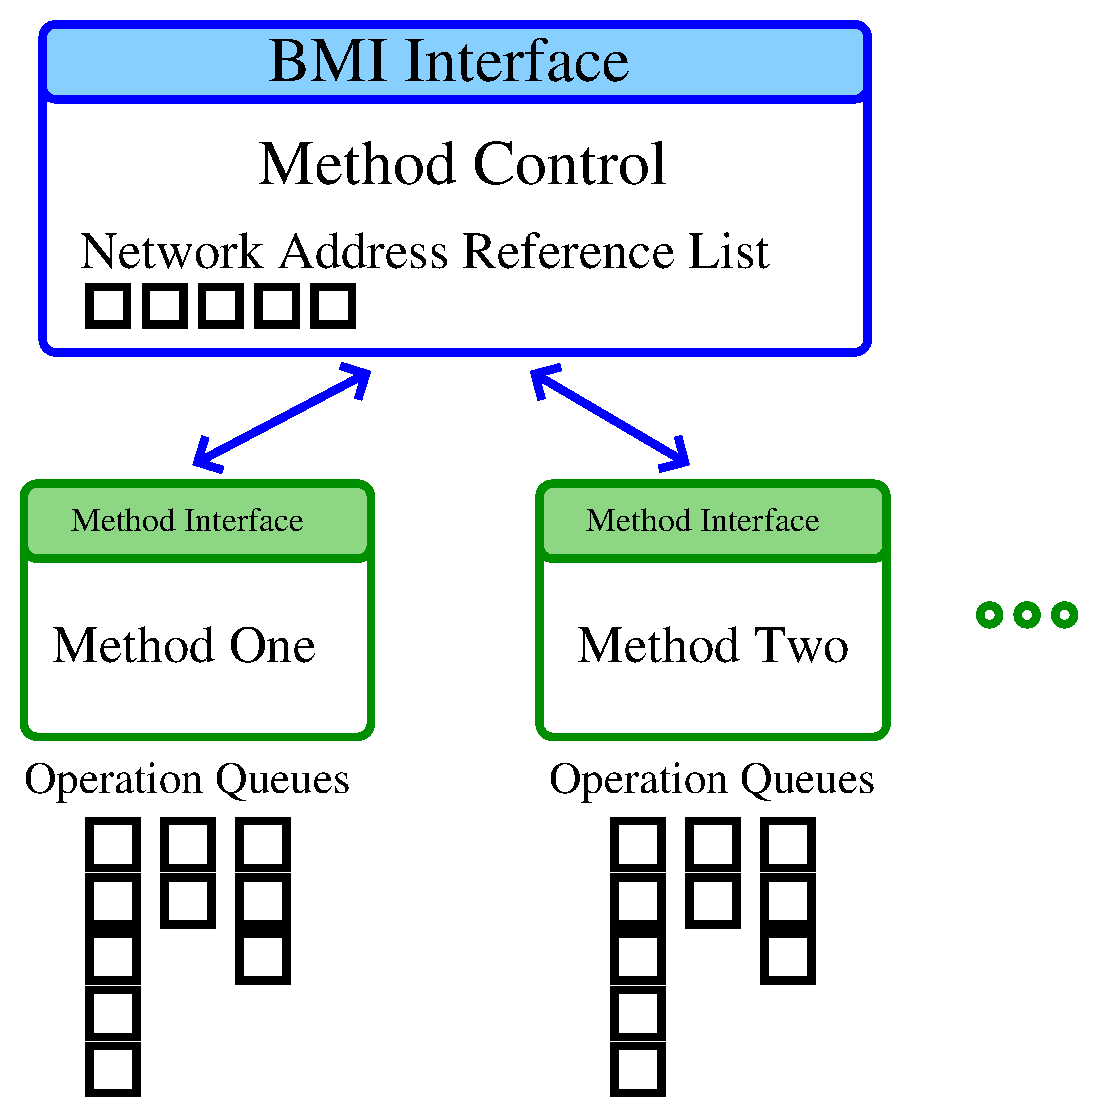
\includegraphics[scale=0.4]{bmi-arch-color.eps}
\end{center}
\caption{BMI Architecture \label{fig:bmi-arch}}
\end{figure}

\subsubsection{Method control}
\label{method-control-intro}

From a high level, the method control layer is responsible for
orchestrating network operations and managing the network methods.
This includes several responsibilities, including address resolution,
method multiplexing, and providing a stable BMI user interface.  It also
provides a library of support functions that may be useful to method
implementors.

One of the most important tasks of the method control layer is the
multiplexing of network methods.  When an operation is
posted by the user, it is up to the method control to decide which
method will service the operation.  Likewise, when the user tests for
completion, the method control must test the appropriate methods for
the operations of interest.

The method control layer provides the BMI user interface.  This is
the API used by applications that communicate using BMI.  The BMI
interface functions are converted into the appropriate low level method
requests that are needed to complete operations.

Address resolution is the final major responsibility of the method
control.  The method control manages the BMI level addresses and makes
sure that the
name space is consistent to the user, regardless of which methods are
in use.  It does so by maintaining an internal \emph{reference list} for
addresses.  Each network address has a unique reference that provides
mappings between BMI user level addresses, the string representation
of addresses, and the method specific representation of addresses.
The BMI user level addresses are handles for network hosts that the
application uses when calling BMI functions.  The string representation
is the ASCII host name of the hosts before they are resolved by BMI (as
read from a ``hosts'' file, for example).
Finally, the method address is the representation that that methods use
for identifying hosts, which may contain information specific
to that particular protocol.  Note that method addresses are never,
under any circumstances, exposed to the application.  They are
reserved for internal BMI use only.

\subsubsection{Methods}

Each method is implemented as a statically compiled module.  This
module must provide (and strictly adhere to) a predefined \emph{method
interface}.  It supports reliable, ordered delivery and flow control for
the protocol that it controls.  Aside from meeting these semantics and
adhering to the method interface, there are no other restrictions on
how the method should be implemented.  Support libraries are provided
for certain features that are common to many methods, but their use
is optional.

Each method is responsible for maintaining the collection of
operations that it is working on, usually through operation queues.
These collections of operations are private to each method.

\subsubsection{Thread safety}

The top level BMI user interface is thread safe.  This means that
it is legal for more than one thread to make concurrent BMI calls,
as long as those calls do not manipulate the same data structures
or operations.  For example, one thread may handle BMI messages to
carry out I/O, while another thread handles BMI messages to
exchange requests and acknowledgements.

The BMI methods do not need to be thread safe.  The method control
layer will serialize any calls to a single method so that it is
protected.  This should ease the process of implementing new
methods.

\section{Concepts}

\subsection{Memory buffers}

The user must specify a memory buffer to use when posting send or
receive operations.  This buffer may be a normal memory region, or it
may be a buffer that was allocated using BMI memory management functions.
If the user elects to allocate the memory using the BMI facilities, then
BMI has the opportunity to optimize the buffer for the type of network
being used.  This mode of operation is preferred for achieving optimal
performance.  However, normal memory buffers are also allowed in order
to better support certain scenarios common to file system operations.
Some file system operations act upon existing memory regions (for example,
the client side Unix read() system call).  In these situations, we would
like to avoid imposing a buffer copy, and instead give the BMI layer
the flexibility to handle the buffer at a lower level if possible.

If a memory buffer is allocated using BMI function calls, then it must
also be deallocated using BMI.  These buffers are not guaranteed to be
manageable by standard operating system libraries.

\subsection{Unexpected messages}
\label{sec:unexp}

BMI's default mode of operation requires that each send operation be
matched with a certain receive operation at the remote host in order to
complete.  This send and receive operation must match in terms of expected
message size (more on this in section \ref{sec:short}), host address,
and identication tag.  Otherwise the communication will not complete.
There is no mechanism for receiving from a ``wildcard'' address.

However, in order to loosen this restriction, 
BMI provides a special class of messages called \emph{unexpected
messages}.   This type of message is sent without the receiving host 
explicitly requesting the communication. 
In other
words, the receiving host does not post a matching receive for this
type of message.  Instead, it must periodically check to see if any
unexpected messages have arrived in order to receive them successfully.
This is the equivalent of ``listening'' for new requests in a more
traditional
networking system.  Unexpected messages may come from any host on the
network.  Communication between two hosts is typically initiated
by one of the hosts sending an unexpected message to the other. 

Unexpected messages may be of any size less than a limit defined by the
interface.  When an unexpected message arrives, BMI will provide a
buffer for it.  This buffer is passed to the receiving process when it
checks to see if unexpected messages have arrived.  It is the
responsibility of the caller to eventually free this buffer using
the normal system free() function.

\subsection{Short messages}
\label{sec:short}

The BMI interface does not allow partial completion of messages.
However, it does allow for a sender to send less data than
the receiver anticipated, resulting in what may be thought of as
``short'' messages from the receiver's point of view.  Short
messages \emph{do not} indicate that another receive is needed to
obtain the rest of the message.  Instead it means that the
sender does not have as much data to transmit as the receiver was
expecting it to.  In practice, this tends to occur in file systems
when a read operation reaches EOF.  It may also be a common
occurance in request protocol operations, when requests may be of
variable size and we do not wish to negotiate the correct size of
messages before transmitting.

When a short send is posted, the sender must indicate the size
that the receiver was expecting.  This is necessary for the
message to be matched properly between sender and receiver.  When
the receive completes, the caller is notified of how much data was
actually present in the message.

\subsection{Immediate completion}

The default model for each network operation is to first post it and
then test for completion.  However, there are often instances in which
operations can complete immediately (during the post procedure) and thus
do not require the extra test step.  Examples of this occur when TCP
sockets buffers are large enough to allow a message to be sent in one step
without blocking.  This may also occur on the receive side of
communications if the required data has already been buffered by the BMI
library when the receive operation is posted.

In these situations, it would be good to avoid the overhead of
needlessly calling the test function.  We therefore allow
\emph{immediate completion} from any post function.  Immediate
completion is indicated from post functions by a return value of one.
BMI library users should always check this return value so that they are
aware of opportunities to skip the test phase of communication.

\subsection{User pointers}

BMI is intended to be used in an enviroment in which many
operations are in flight at once.  Several
operations may be posted at different times for different tasks,
with completion following later in a test() or wait() call.
This sometimes makes it challenging to map the completion of an
operation back to the higher level operation or state that the
user was trying to carry out.

BMI includes the concept of ``user pointers'' to help with this
problem.  A user pointer is a void* passed in to message post
functions, which is returned to the user when the message
completes.  The caller may use these pointer fields for any
purpose.  Typically it will be useful as a mechanism to map back
to a higher level state without having to search through a queue
of operations that are currently in flight.  If used properly,
user pointers eliminate the need for the caller to keep track of
operation id's for any reason other than for calling test()
functions.

\subsection{List I/O}

BMI provides seperate API functions for posting contiguous and
noncontiguous buffers for communication.   Noncontiguous buffers
are represented as arrays of buffer pointers and sizes, and are
handled by functions with the \emph{\_list} suffix.

List I/O is useful when a user wishes to send from or receive data
into multiple memory regions using a single network message.  This
is convenient for mapping network I/O to parallel I/O access patterns.

Messages posted using the list interface are completely compatible
with contiguous messages on the peer side.  Regions do not have to
match between sender and receiver, nor do they both have to be
discontiguous.  The aggregate size of the message does need to
match, however.
The list functions support all of the features of the ``normal''
API, including short messages.

The intention is for method level support of list messages to be
optional; if a method does not implement this functionality, then
the method control layer of BMI will emulate it by packing and
unpacking regions using contiguous intermediate buffers.  This is
obviously a performance penalty, but will ensure correct behavior
when a native method cannot easily handle discontiguous memory
regions.

\section{User interface}
\label{sec:user}

\subsection{Types and structures}

\begin{itemize}

\item \textbf{Message tags}:  Message tags are numerical values that may
be associated with messages to be sent or received using BMI.  The
sending and receiving process must use matching tags in order for a
given communication to complete.  Unexpected messages are the only
exception; in that case only the sender must specify a tag.  

Tags provide a mechanism for PVFS to differentiate between various
messages and associate them with specific tasks.

\item \textbf{ID's}:  ID's are opaque handles that a caller may use to
keep track of operations that are currently in progress.  ID's are
assigned by BMI when an operation is posted and then used in subsequent tests
to determine if the operation has completed.

\item \textbf{unexpected\_info}: This is a struct used to
describe incoming unexpected messages.  It is filled in by the
testunexpected() and waitunexpected() calls (see below).

\end{itemize}

\subsection{Interface functions}

The BMI interface can be separated into categories as follows:  message
initiation, message testing, memory management, list I/O, and utilities. 

The message initiation functions are used by an application to 
request the sending or receiving of network buffers:

\begin{itemize}
\item \textbf{BMI\_post\_send()}: Posts a send operation.
\item \textbf{BMI\_post\_recv()}: Posts a receive operation.
\item \textbf{BMI\_post\_sendunexpected()}: Posts a send operation
that was not expected by the receiving process.
\item \textbf{BMI\_unpost()}: Unposts a previously submitted
operation.  \emph{This is a blocking call.}
\item \textbf{BMI\_addr\_lookup()}: Converts the string
representation of a BMI address (in url-like form) into an opaque
BMI addr type.
\end{itemize}

The message testing functions are used to check for completion of
network operations:

\begin{itemize}

\item \textbf{BMI\_test()}: Tests for completion of a single
operation.
\item \textbf{BMI\_testsome()}: Tests for completion of any of a
specified set of operations.
\item \textbf{BMI\_testunexpected()}: Tests for arrival of any
unexpected messages.
\item \textbf{BMI\_wait()}:  Tests for completion of a single
operation; is allowed to block briefly if no work is available.
\item \textbf{BMI\_waitsome()}: Tests for completion of any of a
specified set of operations; is allowed to block briefly if no
work is available.
\item \textbf{BMI\_waitunexpected()}: Tests for completion of any
of a specified set of operations; is allowed to block briefly if
no work is available.
\end{itemize}

The BMI memory management functions are used to control memory buffers
that are optimized for use with BMI:

\begin{itemize}

\item \textbf{BMI\_memalloc()}:  Creates a new buffer. 
\item \textbf{BMI\_memfree()}:  Destroys a buffer previously
created with BMI\_memalloc().

\end{itemize}

The list I/O functions are very similar to the message initiation
functions.  However, they allow the caller to express buffers as
arrays of discontiguous regions

Note that each of these functions requires the caller to pass in
an array of pointers and sizes to use as I/O targets.  These
arrays must not be freed or modified until completion of the
requested operation (they are not copied by the BMI interface).

\begin{itemize}
\item \textbf{BMI\_post\_send\_list()}:  Same as BMI\_post\_send,
except that it allows the caller to specify an array of buffers
and sizes to send from.
\item \textbf{BMI\_post\_recv\_list()}:  Same as BMI\_post\_recv,
except that it allows the caller to specify an array of buffers
and sizes to receive into.
\item \textbf{BMI\_post\_sendunexpected\_list()}:  Same as
BMI\_post\_sendunexpected(), execept that it allows the caller to
specify an array of buffers and sizes to send from.
\end{itemize}

The final collection of functions perform various utility tasks that are
not directly involved in network I/O:

\begin{itemize}

\item \textbf{BMI\_initialize()}:  Starts the BMI interface; must
be called prior to any other BMI functions.
\item \textbf{BMI\_finalize()}:  Shuts down the BMI interface.
\item \textbf{BMI\_set\_info()}:  Sets optional BMI parameters.
\item \textbf{BMI\_get\_info()}:  Reads optional BMI parameters.

\end{itemize}

\subsubsection{Supported getinfo and setinfo options}

\begin{itemize}
\item BMI\_DROP\_ADDR: This is a hint which may be passed to
set\_info.  It tells the interface that no further communication
will be requested of the specified address, and that it should be
discarded.  \emph{NOTE: this option will almost certainly be
deprecated or replaced soon}
\item BMI\_CHECK\_INIT: This is a query to get\_info which simply
checks to see if the BMI interface has been properly initialized
or not.
\end{itemize}

\subsection{Error handling}

Errors may be reported from BMI in one of two ways:

\begin{itemize}
\item \emph{Return value of API function}:  If an API function
returns a value less than zero, it indicates that the function
failed.  This is an indication of a critical internal error that
is not particular to any specific operation.
\item \emph{Operation error code}:  This is a value filled in upon
completion of an operation.  If less than zero, it indicates that
the operation in question failed, but that the BMI interface as a
whole is working properly.
\end{itemize}

Both types of error codes for the time being consist of -errno
values.  This is not really expressive enough for long term use,
but at least gives a general idea of the type of failure for now.

\section{Method implementation}
\label{sec:methguide}

The method interface is very similar to the BMI user interface.
It implements roughly the same functions. However, it includes minor
variations that take into account the fact that operations at this level
are targeted for a single specific method.

\subsection{Method interface}

\begin{itemize}

\item \textbf{BMI\_method\_initialize()}:
\item \textbf{BMI\_method\_finalize()}:
\item \textbf{BMI\_method\_post\_send()}:
\item \textbf{BMI\_method\_post\_sendunexpected()}:
\item \textbf{BMI\_method\_post\_recv()}:
\item \textbf{BMI\_method\_unpost()}: 
\item \textbf{BMI\_method\_addr\_lookup()}:
\item \textbf{BMI\_method\_test()}: 
\item \textbf{BMI\_method\_testsome()}: 
\item \textbf{BMI\_method\_testunexpected()}:
\item \textbf{BMI\_method\_wait()}: 
\item \textbf{BMI\_method\_waitsome()}: 
\item \textbf{BMI\_method\_waitunexpected()}:
\item \textbf{BMI\_method\_memalloc()}:
\item \textbf{BMI\_method\_memfree()}:
\item \textbf{BMI\_method\_set\_info()}:
\item \textbf{BMI\_method\_get\_info()}:
\item \textbf{BMI\_method\_post\_send\_list()}:
\item \textbf{BMI\_method\_post\_sendunexpected\_list()}:
\item \textbf{BMI\_method\_post\_recv\_list()}:

\end{itemize}

\subsection{Important structures}

There are three major structures that are manipulated at the BMI
method level API:

\begin{itemize}
\item \textbf{method\_op}:  This structure is used to keep track
of pending operations.  It includes several generic fields which
should apply to almost any method, as well as a private area which
may be used internally by methods for storage of parameters.
\item \textbf{method\_addr}:  This structure is used to describe
network addresses at the method level.  Like the method\_op
structure, it has both generic and private sections.
\item \textbf{method\_unexpected\_info}: This structure describes
incoming unexpected messages.  It is filled in during
testunexpected(), and converted into information to be passed to
the BMI user by the method control layer.
\end{itemize}

\subsection{Support libraries}
\label{sec:support}

The BMI library provides several support functions which may aid
method programmers when implementing support for new protocols.  Each
method can expect these functions to be visible to it once it has been
linked into the library.
These functions are
intended to be as generic as possible so that they may be used by a
variety of different methods.

\subsubsection{Operation queues}

Every prototype method implemented so far makes use of FIFO queues to
keep track of pending operations.  Operations are described by generic
operation structures that include common parameters (such as buffer
size and location).  This structure also includes abstract storage space
for private method specific parameters (such as flow control or device
management information).  The operation queue mechanism in BMI is based
on the doubly linked list implementation found in the Linux kernel. 

\begin{itemize}
\item \textbf{op\_queue\_new()}: Creates a new operation queue.
\item \textbf{op\_queue\_cleanup()}:  Destroys an existing
operation queue as well as any operations contained within it.
\item \textbf{op\_queue\_add()}:  Adds a
method operation onto the tail of a queue.
\item \textbf{op\_queue\_remove()}:  Removes a specific
operation from the queue in which it resides.
\item \textbf{op\_queue\_search()}:  Searches for
an operation that matches the characteristics specified a given key.  All
searches begin at the head of the target operation queue.
\item \textbf{op\_queue\_empty()}: Determines whether a
queue is empty or not.
\item \textbf{op\_queue\_count()}: Counts the number of
entries within an operation queue.  This function requires iteration
through every element of the queue.  It is therefore only suitable for
debugging purposes in which performance is not critical.
\item \textbf{op\_queue\_dump()}: Prints out
information about every operation in the queue.  Only used for debugging
and prototyping purposes.
\end{itemize}

Two related functions are also provided for managing the creation of
operation structures:

\begin{itemize}
\item \textbf{alloc\_method\_op()}:  Allocates a new
operation structure.
\item \textbf{dealloc\_method\_op()}: Deallocates an existing
method operation.
\end{itemize}

\subsubsection{Method address support}

Method address structures are used by methods to identify network hosts.
Like operation structures, they contain private storage for internal
method use.  Three functions are provided to aid in managing these
structures:

\begin{itemize}
\item \textbf{alloc\_method\_addr()}:  Creates
a new address structure.  
\item \textbf{dealloc\_method\_addr()}:  Destroys an
existing method address structure.
\item \textbf{bmi\_method\_addr\_reg\_callback()}:
This is called by a method to inform the method control layer that it
should register a new method address structure.  The function is
typically invoked when an unexpected message arrives and the method must
create a new address structure to represent the source
host and register it with the upper API layers.  
\end{itemize}

\subsubsection{Logging and debugging}

BMI uses the \emph{gossip} library for reporting errors and
logging messages.  This mechanism is used in several other
components besides BMI as well.  A discussion of gossip may be
found in the \emph{parl-developer-guidelines} document.

\subsubsection{Operation id's}

Each method is responsible for creating opaque id's that can be used to
refer to operations that are currently in progress.  Typically these
id's will be used to map user requests to specific operation structures.
The \emph{id\_generator} library is available to aid methods in
performing this mapping operation.  It
also insures that the id space is consistent across all methods.

\begin{itemize}
\item \textbf{id\_gen\_fast\_register()}: Registers
a new structure with the interface and creates a new id that may be used
to reference it.
\item \textbf{id\_gen\_fast\_lookup()}:  Returns a pointer to the
original data structure that was associated with the given id.
\end{itemize}

\section{References}
\label{sec:ref}

\begin{itemize}
\item \textbf{source code}: The source code to BMI may be found in the
``pvfs2'' cvs tree, within the pvfs2/src/io/bmi directory.
\item \textbf{example methods}: Two example methods have been created
thus far.  A method for the GM protocol may be found in
pvfs2/src/io/bmi/bmi\_gm.  A method for the TCP/IP protocol may be found
in pvfs2/src/io/bmi/bmi\_tcp.
\item \textbf{benchmarks}:  Benchmarks that compare MPI and BMI
can be found in pvfs2/src/io/bmi/benchmark.   
\item \textbf{example applications}:  Example applications that use BMI
directly may be found in pvfs2/src/io/bmi/examples.   
\item \textbf{BMI technical paper}: work in progress, available in
cvs as the ``bmi\_paper'' project.
\end{itemize}


\end{document}

